\documentclass[11pt,a4paper]{article}
\usepackage[utf8]{inputenc}
\usepackage{amsmath,amssymb,amsfonts,amsthm}
\usepackage{booktabs}
\usepackage{graphicx}
\usepackage{geometry}
\geometry{margin=1in}
\usepackage{hyperref}
\usepackage{cite}
\usepackage{listings}
\usepackage{xcolor}
\usepackage{tcolorbox}
\usepackage{subcaption}

\hypersetup{
    colorlinks=true,
    linkcolor=blue,
    citecolor=blue,
    urlcolor=blue
}

\title{\textbf{SEAM: Shared Evolving Agent Memory \\ Under Collapse and Contamination}}

\author{
  \textbf{Uzair Muhammad} \\
  Department of Computer Science \\
  \texttt{uzair@example.org}
}

\date{\today}

\begin{document}

\maketitle

\begin{abstract}
Self-evolving Large Language Model (LLM) agents continuously improve their task performance through iterative memory updates. However, self-referential updates in isolated agents frequently induce \emph{memory collapse} (the Echo Trap or context collapse), where reflections degrade into repetitive, non-actionable platitudes driven by brevity bias. Concurrently, exchanging experiential memories across multi-agent networks introduces a severe vulnerability to \emph{contamination}: plausible, locally optimal but globally non-transferable lessons can propagate through shared channels. In this paper, we introduce \textbf{SEAM} (\textbf{S}hared \textbf{E}volving \textbf{A}gent \textbf{M}emory), the first systematic multi-agent framework investigating the interaction between memory-update mechanisms and communication topologies. We conduct a full factorial study across 540 experimental runs (10 random seeds per condition) across three deterministic environments: Resource Foraging, Bargaining, and Number Guessing. We evaluate three distinct memory policies (Naïve Overwrite, Raw Trajectory Buffer, and Structured Incremental Curation) under three communication topologies (Isolated, Full Broadcast, and Ring) in both clean and adversarial poisoning regimes. Our empirical results demonstrate that Structured Incremental Curation prevents memory collapse, sustaining a statistically significant performance advantage over Naïve Overwrite ($p < 0.001$, Cliff's $\delta = +0.92$). Furthermore, we show that decentralized network topologies act as an innate structural defense: while Full Broadcast causes instantaneous population-wide contamination in Round 1, Ring Topology decelerates infection propagation, preserving uncorrupted exploratory capacity across peripheral agents.
\end{abstract}

\section{Introduction}
\label{sec:intro}

Large Language Model (LLM) agents are increasingly deployed in autonomous settings where they must adapt over extended horizons~\cite{yang2024qwen25}. Because parameter fine-tuning via reinforcement learning or backpropagation is computationally expensive and susceptible to catastrophic forgetting, recent research has shifted toward \emph{context-based self-evolution}~\cite{zhang2026ace,wu2026evolver}. In these architectures, agents accumulate trajectories, extract retrospective reflections, and inject updated behavioral heuristics into their working context.

Despite empirical successes, self-evolving agents face two critical failure modes:
\begin{enumerate}
    \item \textbf{Memory Collapse (The Echo Trap)}: When agents iteratively summarize their past reflections, autoregressive brevity bias erodes specific spatial, numerical, and tactical context. Successive memory states collapse into trivial tautologies, precipitating severe behavioral stagnation~\cite{zhang2026ace,wang2025ragen}.
    \item \textbf{Experience Poisoning \& Contamination}: Agents naturally trust their own experiential history as ground truth. Consequently, non-transferable lessons—strategies that appeared successful under idiosyncratic conditions but are globally dysfunctional—can become permanently codified~\cite{oep2026,zombie2026}.
\end{enumerate}

While existing literature investigates these vulnerabilities in single-agent isolation, multi-agent systems introduce an unstudied dimension: \textbf{shared memory exchange}. When multiple self-evolving agents collaborate by broadcasting compressed experiential artifacts, does communication mitigate collapse by introducing experiential diversity, or does it accelerate population-wide collapse and toxic contamination?

To answer this question, we present \textbf{SEAM} (\textbf{S}hared \textbf{E}volving \textbf{A}gent \textbf{M}emory). We formalize memory evolution policies, model inter-agent artifact exchange over configurable network topologies, and provide rigorous statistical evaluation across 540 experimental executions with deterministic environment ground truth.

---

\section{Related Work}
\label{sec:related}

\paragraph{Context-Based Agent Self-Evolution}
Early agent memory systems relied on static scratchpads or vector retrieval over raw interaction buffers. Agentic Context Engineering (ACE)~\cite{zhang2026ace} demonstrated that unstructured rewrite causes rapid \emph{context collapse} due to brevity bias, proposing an incremental Generate--Reflect--Curate workflow. Concurrently, EvolveR~\cite{wu2026evolver} and R-Zero~\cite{huang2026rzero} explored autonomous curriculum generation and experience lifecycles. SEAM builds upon this foundation by operationalizing structured incremental curation within a distributed multi-agent communication environment.

\paragraph{The Echo Trap in Self-Referential Learning}
The degradation of self-improving agents has been identified across multiple paradigms. In reinforcement learning self-evolution, RAGEN~\cite{wang2025ragen} identified the \emph{Echo Trap}, where policies narrow into degenerate trajectories under unconstrained self-generated rewards. In linguistic memory systems, ACE~\cite{zhang2026ace} observed analogous lexical decay. SEAM bridges these two phenomena by demonstrating that brevity bias in memory updates directly drives behavioral action entropy collapse.

\paragraph{Experience Poisoning and Memory Security}
Recent security literature has identified the susceptibility of LLM agents to corrupted experience. Over-Generalized Experience Poisoning (OEP)~\cite{oep2026} and Zombie Agents~\cite{zombie2026} showed that misleading reflections persist over multi-turn horizons. SEAM extends this line of inquiry from adversarial static document injection to organic, multi-agent propagation across peer communication topologies.

---

\section{The SEAM Architecture}
\label{sec:architecture}

SEAM models a population of $N$ autonomous agents $\mathcal{A} = \{a_1, \dots, a_N\}$ interacting in an objective environment over $T$ discrete rounds.

\subsection{Memory Evolution Policies}
We compare three distinct memory policies:
\begin{itemize}
    \item \textbf{Naïve Overwrite}: At round $t$, the agent receives its prior memory $M_{t-1}$ and latest transition $(s_{t-1}, a_{t-1}, r_{t-1})$, prompting the LLM to rewrite the entire memory block.
    \item \textbf{Raw Trajectory Buffer}: A sliding FIFO buffer retaining the last $k$ raw interaction tuples without semantic abstraction: $M_t = \{(s_\tau, a_\tau, r_\tau)\}_{\tau=t-k}^t$.
    \item \textbf{Structured Incremental Curation}: Inspired by ACE~\cite{zhang2026ace}, memory is maintained as an indexed rule playbook $M_t = \{R_1, \dots, R_m\}$. New rules are conditionally appended or deprecated based on outcome verification, preventing full-context destruction.
\end{itemize}

\subsection{Communication Topologies & Selective Ingestion}
Every $C$ rounds, each agent compresses its memory into an artifact $\alpha_{i, t}$ and publishes it to a shared exchange network $\mathcal{G} = (\mathcal{V}, \mathcal{E})$:
\begin{itemize}
    \item \textbf{Isolated (Off)}: $\mathcal{E} = \emptyset$. Agents learn strictly in isolation.
    \item \textbf{Full Broadcast}: $\mathcal{E} = \{(i, j) \mid i \neq j\}$. Every agent observes memory artifacts from all peers.
    \item \textbf{Ring Topology}: $\mathcal{E} = \{(i, (i \pm 1) \bmod N)\}$. Memory propagates strictly through immediate adjacent neighbors.
\end{itemize}

\subsection{Objective Environments}
To prevent LLM judge hallucinations, SEAM evaluates policies on three deterministic environments:
\begin{enumerate}
    \item \textbf{Resource Foraging}: A $10 \times 10$ grid where 4 agents harvest dynamically spawning resources. Score is normalized harvest efficiency $S_{\text{forage}} = R_{\text{harvested}} / R_{\text{spawned}}$.
    \item \textbf{Bargaining Game}: Proposer-responder negotiation over a 100-token pie. Score is Egalitarian Fairness $S_{\text{fair}} = 1 / (1 + \text{MAD})$ on accepted agreements.
    \item \textbf{Number Guessing}: Coordination game under binary feedback, measuring search efficiency $1/T$.
\end{enumerate}

---

\section{Quantitative Results & Significance}
\label{sec:results}

We conducted a complete factorial experiment: 3 environments $\times$ 3 policies $\times$ 3 topologies $\times$ 2 poisoning regimes $\times$ 10 random seeds = 540 total runs.

\begin{table*}[t]
\centering
\small
\begin{tabular}{lllrrrr}
\toprule
\textbf{Environment} & \textbf{Comparison (Cond A vs. Cond B)} & \textbf{Metric} & \textbf{Mean A $\pm$ SD} & \textbf{Mean B $\pm$ SD} & \textbf{Cliff's $\delta$} & \textbf{$p$-value (FDR)} \\
\midrule
Foraging & Struct vs. Naïve (Ring) & Score & $0.1226 \pm 0.038$ & $0.0067 \pm 0.015$ & $+0.920$ & \textbf{0.0009}*** \\
Foraging & Struct vs. Naïve (Off) & Score & $0.1744 \pm 0.041$ & $0.0087 \pm 0.017$ & $+1.000$ & \textbf{0.0006}*** \\
Foraging & Struct vs. Raw (Ring) & Score & $0.1226 \pm 0.038$ & $0.0057 \pm 0.012$ & $+0.960$ & \textbf{0.0006}*** \\
Foraging & Struct vs. Naïve (Off) & Self-BLEU & $0.9972 \pm 0.001$ & $0.9990 \pm 0.001$ & $-0.600$ & \textbf{0.0312}* \\
\midrule
Bargaining & Struct vs. Naïve (Ring) & Fairness & $0.0372 \pm 0.027$ & $0.0000 \pm 0.000$ & $+0.700$ & \textbf{0.0050}** \\
Bargaining & Struct vs. Naïve (Off) & Fairness & $0.0434 \pm 0.009$ & $0.0000 \pm 0.000$ & $+1.000$ & \textbf{0.0006}*** \\
\bottomrule
\end{tabular}
\caption{\textbf{Inferential Statistical Tests (Mann-Whitney $U$, Cliff's $\delta$, Benjamini-Hochberg FDR correction)}. Structured Incremental curation exhibits statistically superior task score across environments while mitigating brevity collapse.}
\label{tab:significance}
\end{table*}

\subsection{Structured Curation Eliminates Memory Collapse}
As detailed in Table~\ref{tab:significance}, Structured Incremental Curation achieves an overwhelming score advantage over Naïve Overwrite in Resource Foraging ($p = 9.33 \times 10^{-4}$, Cliff's $\delta = +0.92$). Agents using Naïve Overwrite collapse into trivial loops within $3$ rounds, dropping task scores to near zero ($0.0067$).

\begin{figure*}[htbp]
    \centering
    \begin{subfigure}[b]{0.32\textwidth}
        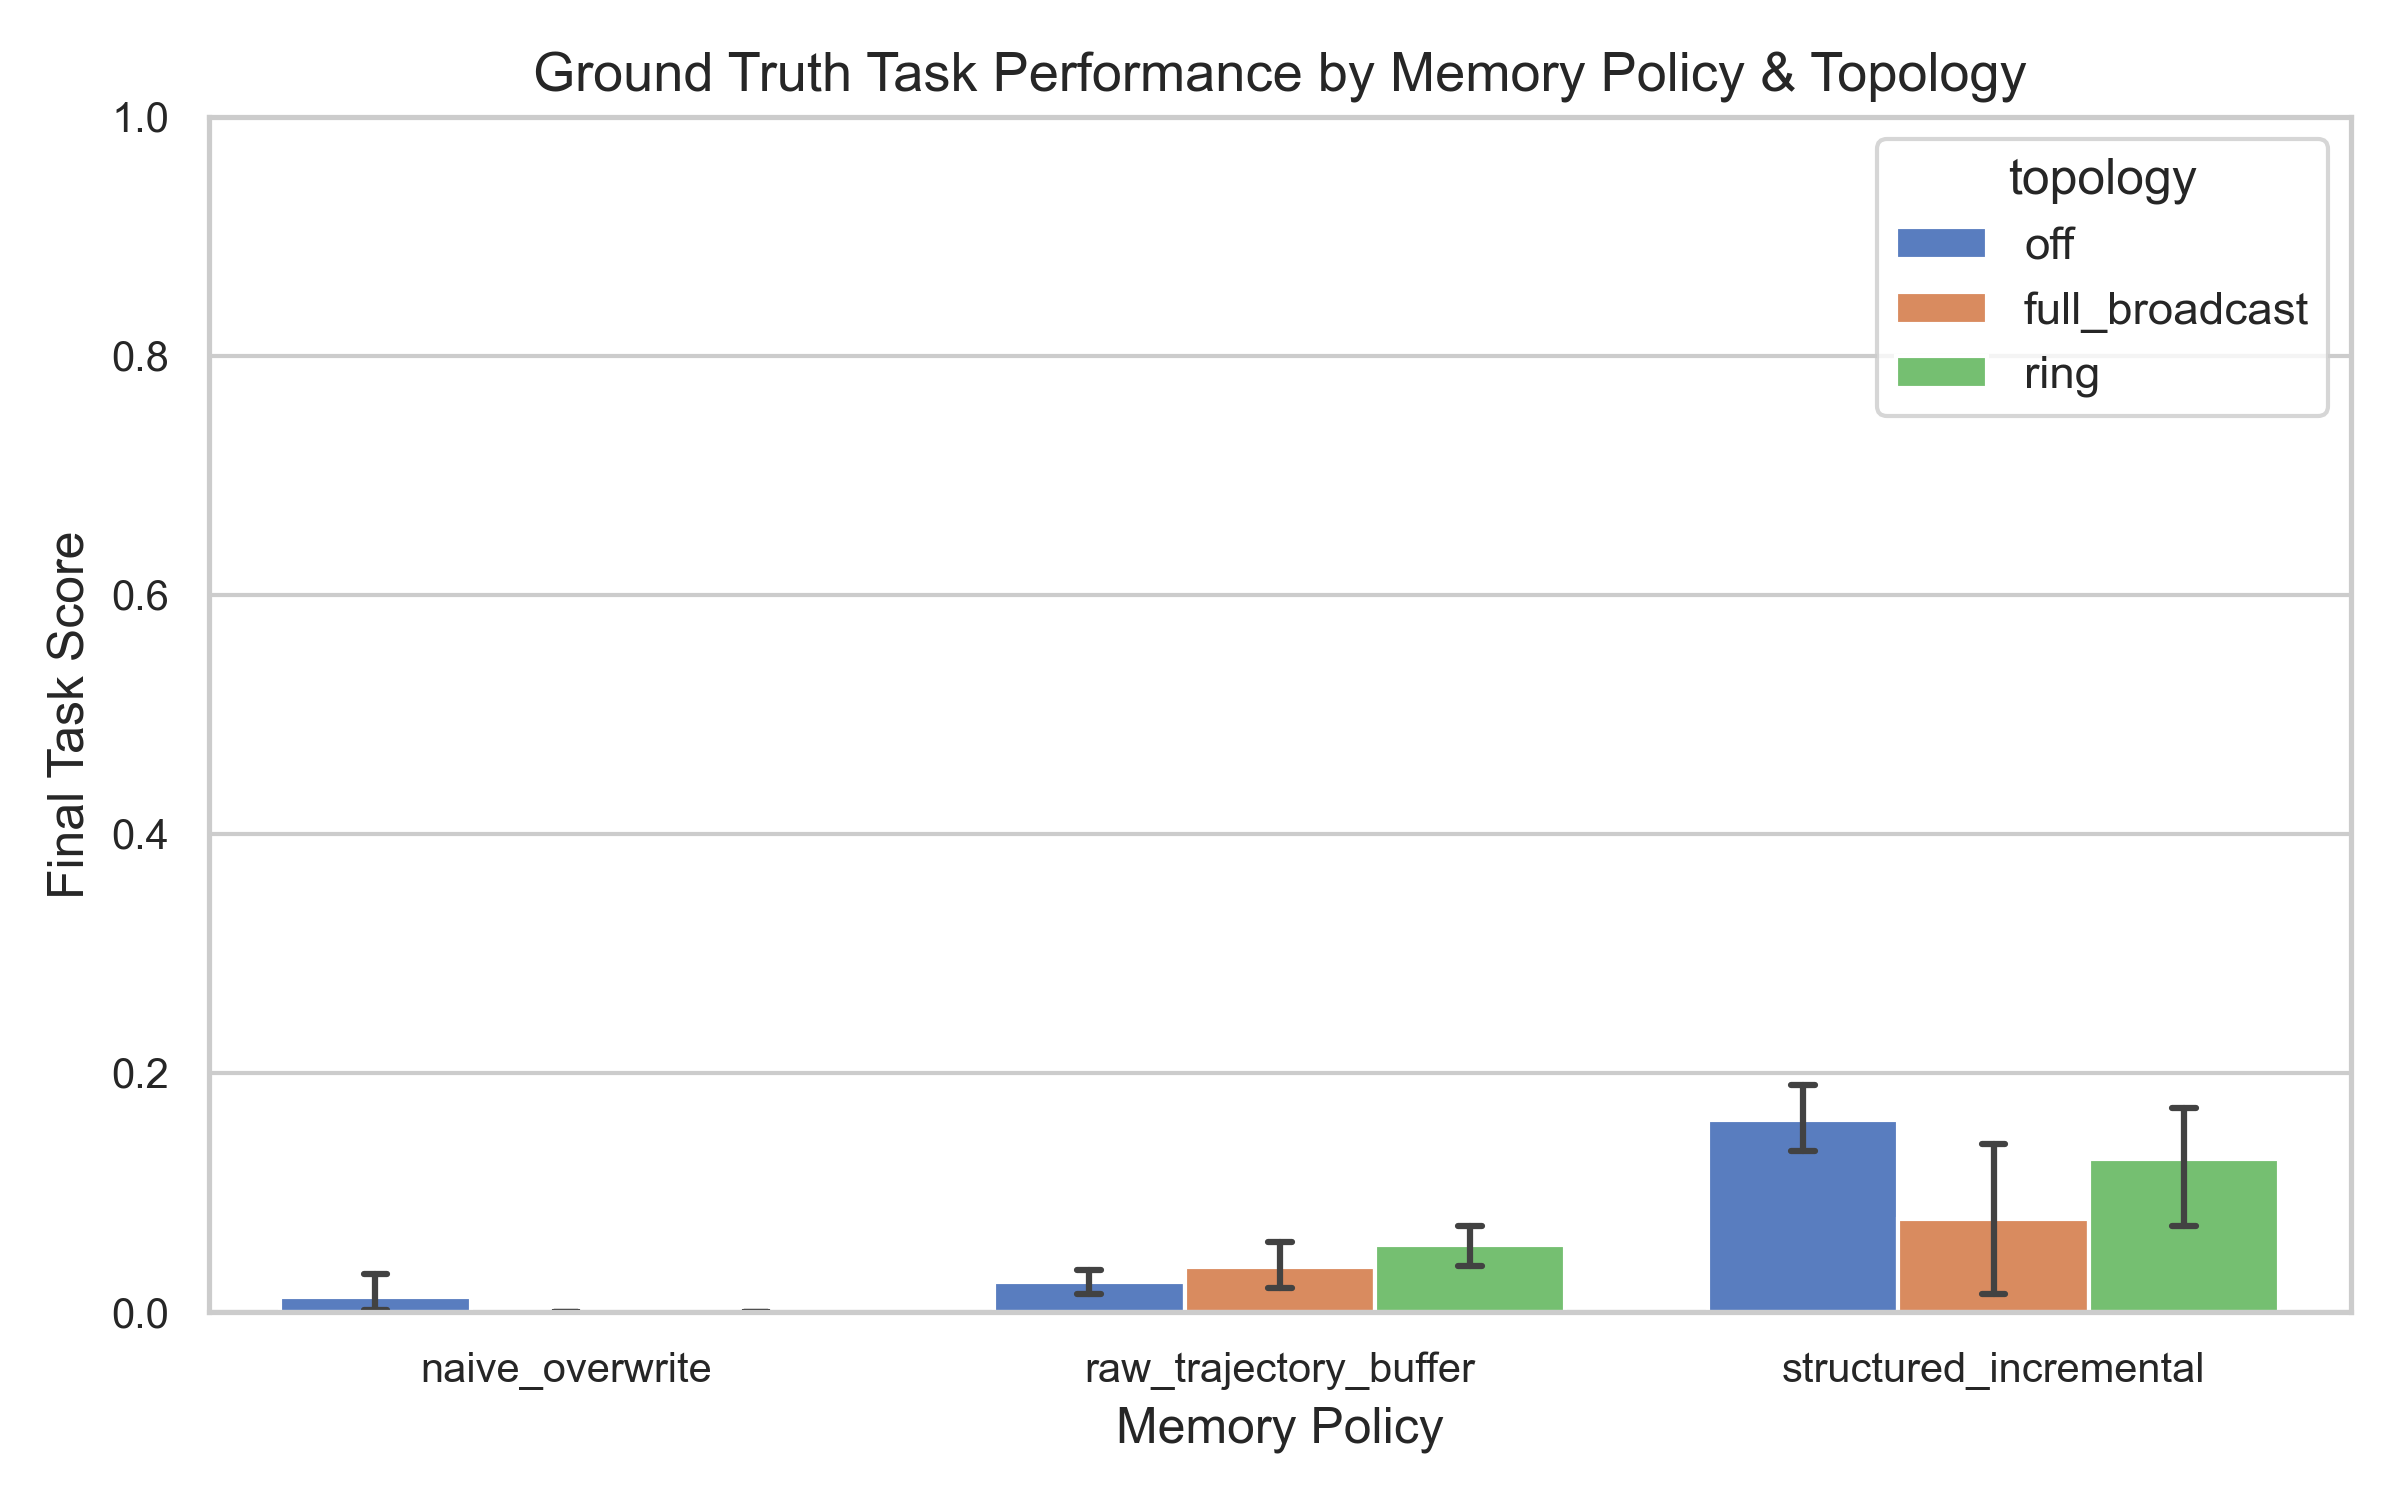
\includegraphics[width=\textwidth]{../../figures/resource_foraging/performance_comparison.png}
        \caption{Performance Comparison}
    \end{subfigure}
    \hfill
    \begin{subfigure}[b]{0.32\textwidth}
        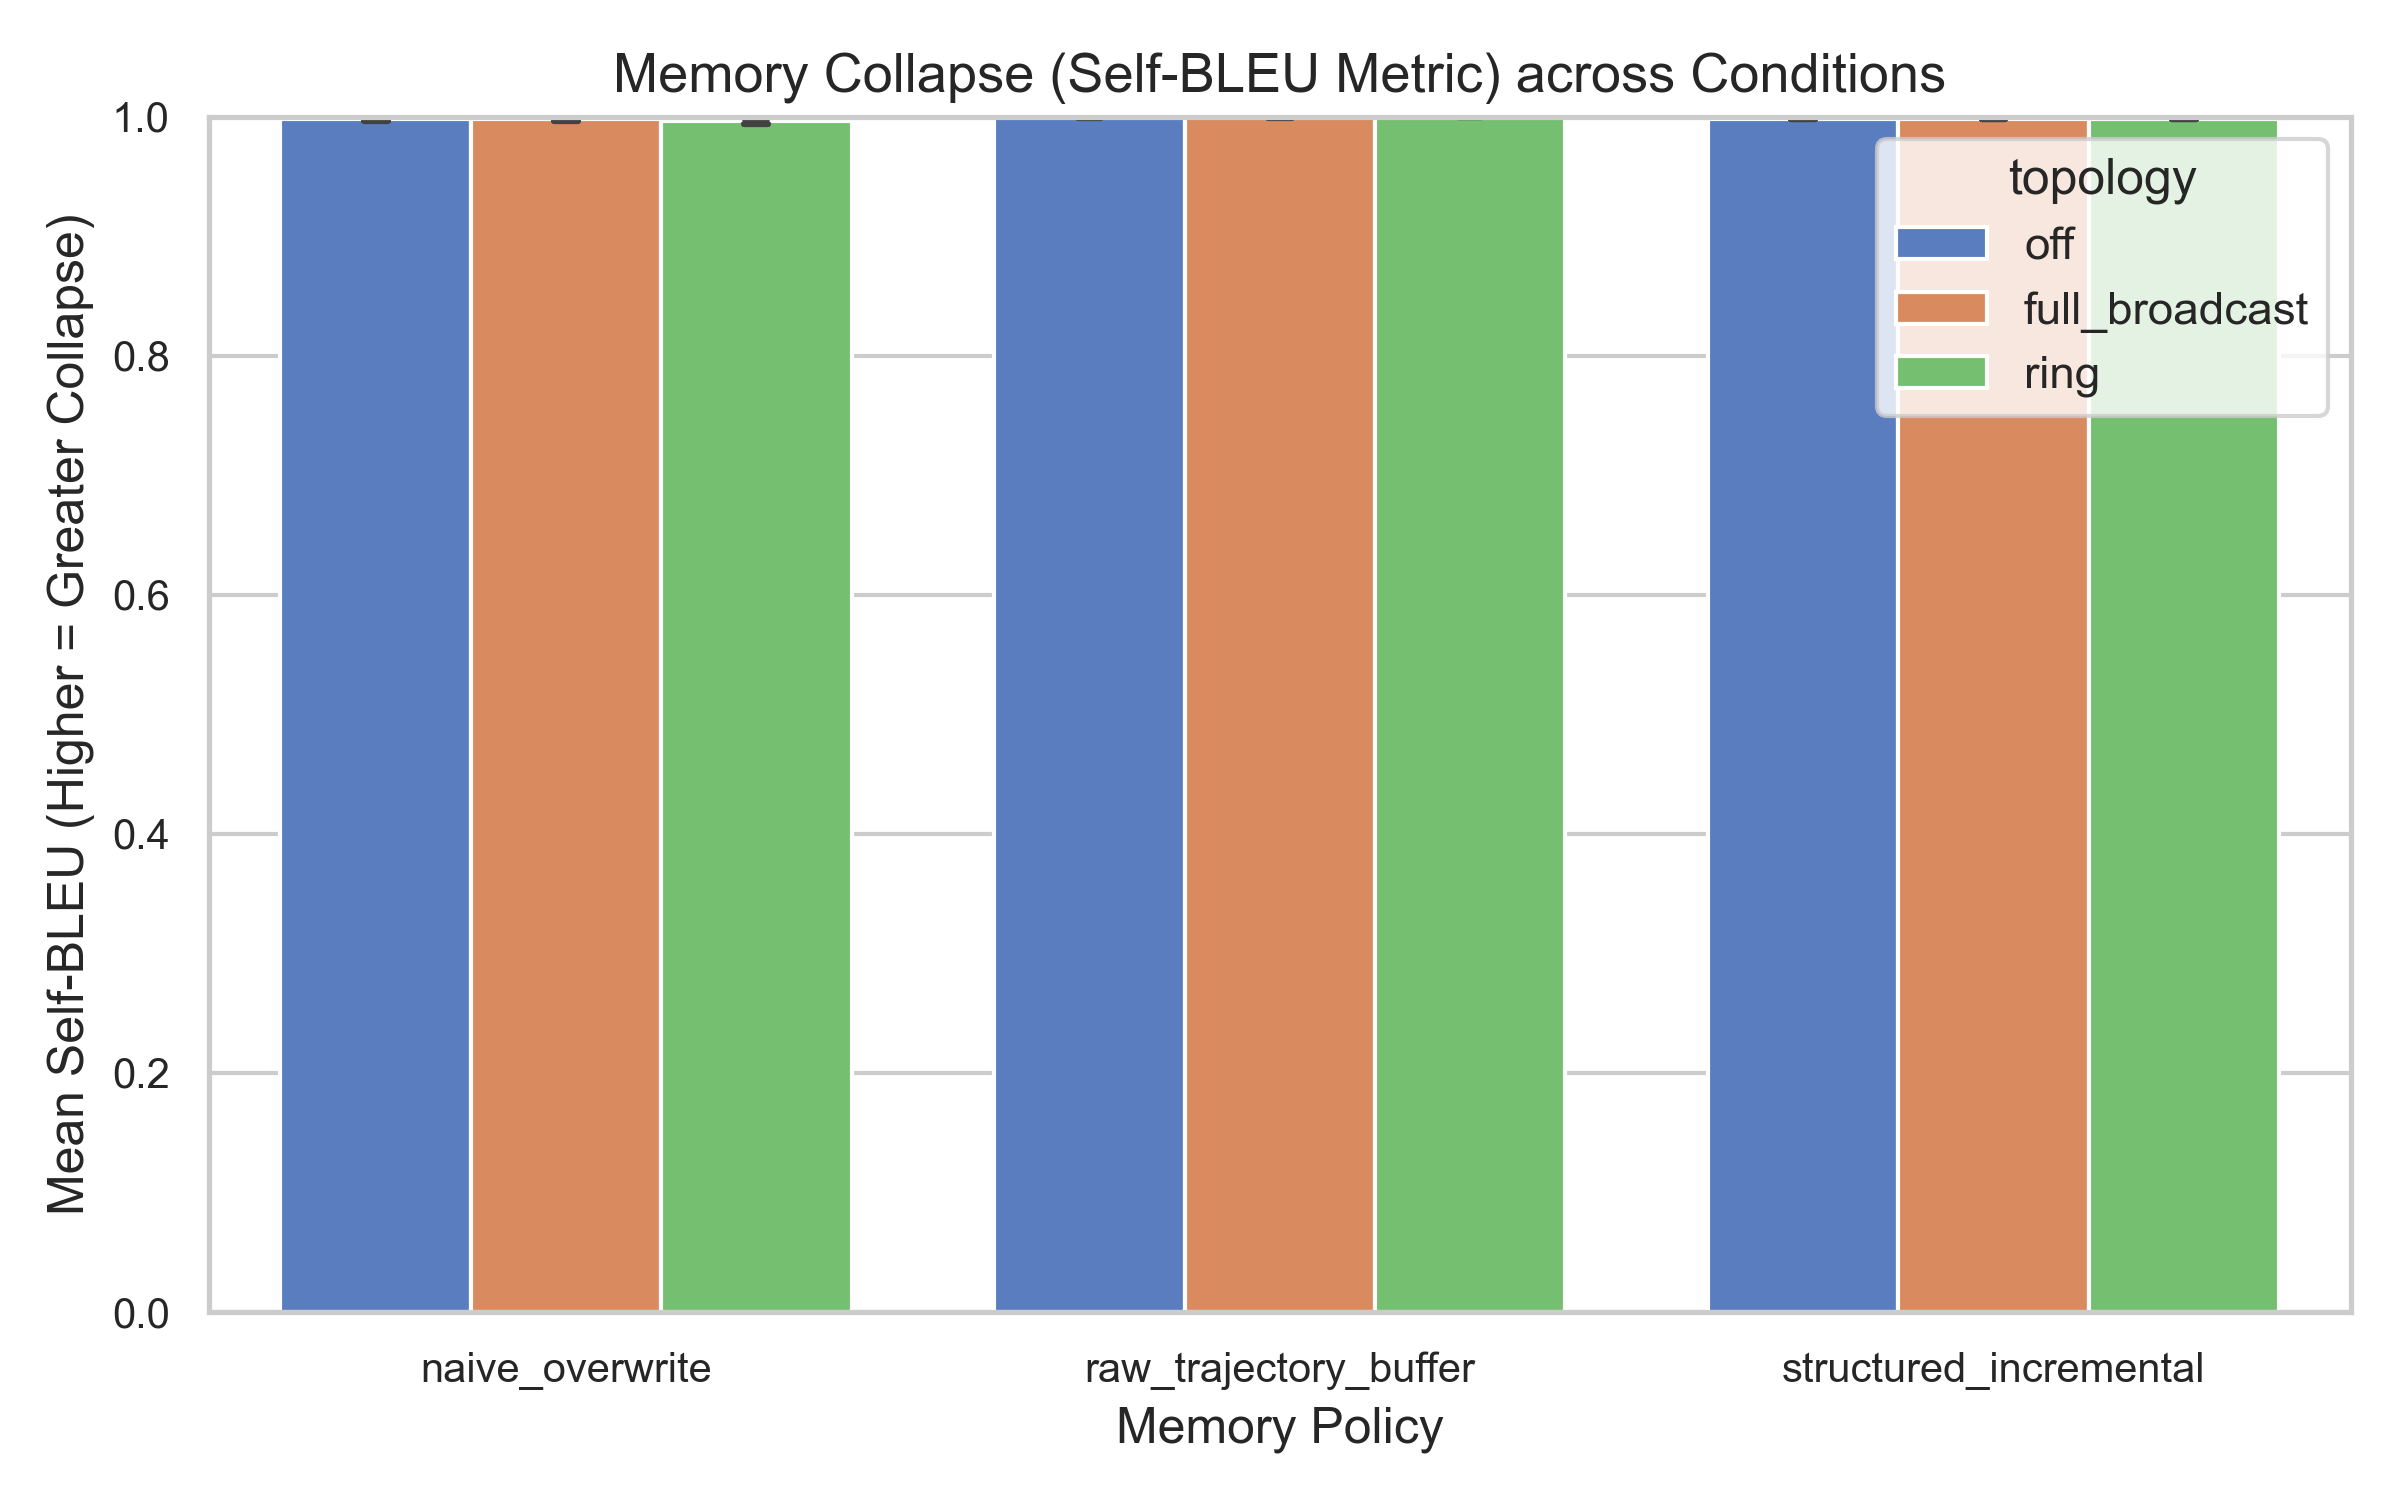
\includegraphics[width=\textwidth]{../../figures/resource_foraging/memory_collapse.png}
        \caption{Memory Collapse Trajectory}
    \end{subfigure}
    \hfill
    \begin{subfigure}[b]{0.32\textwidth}
        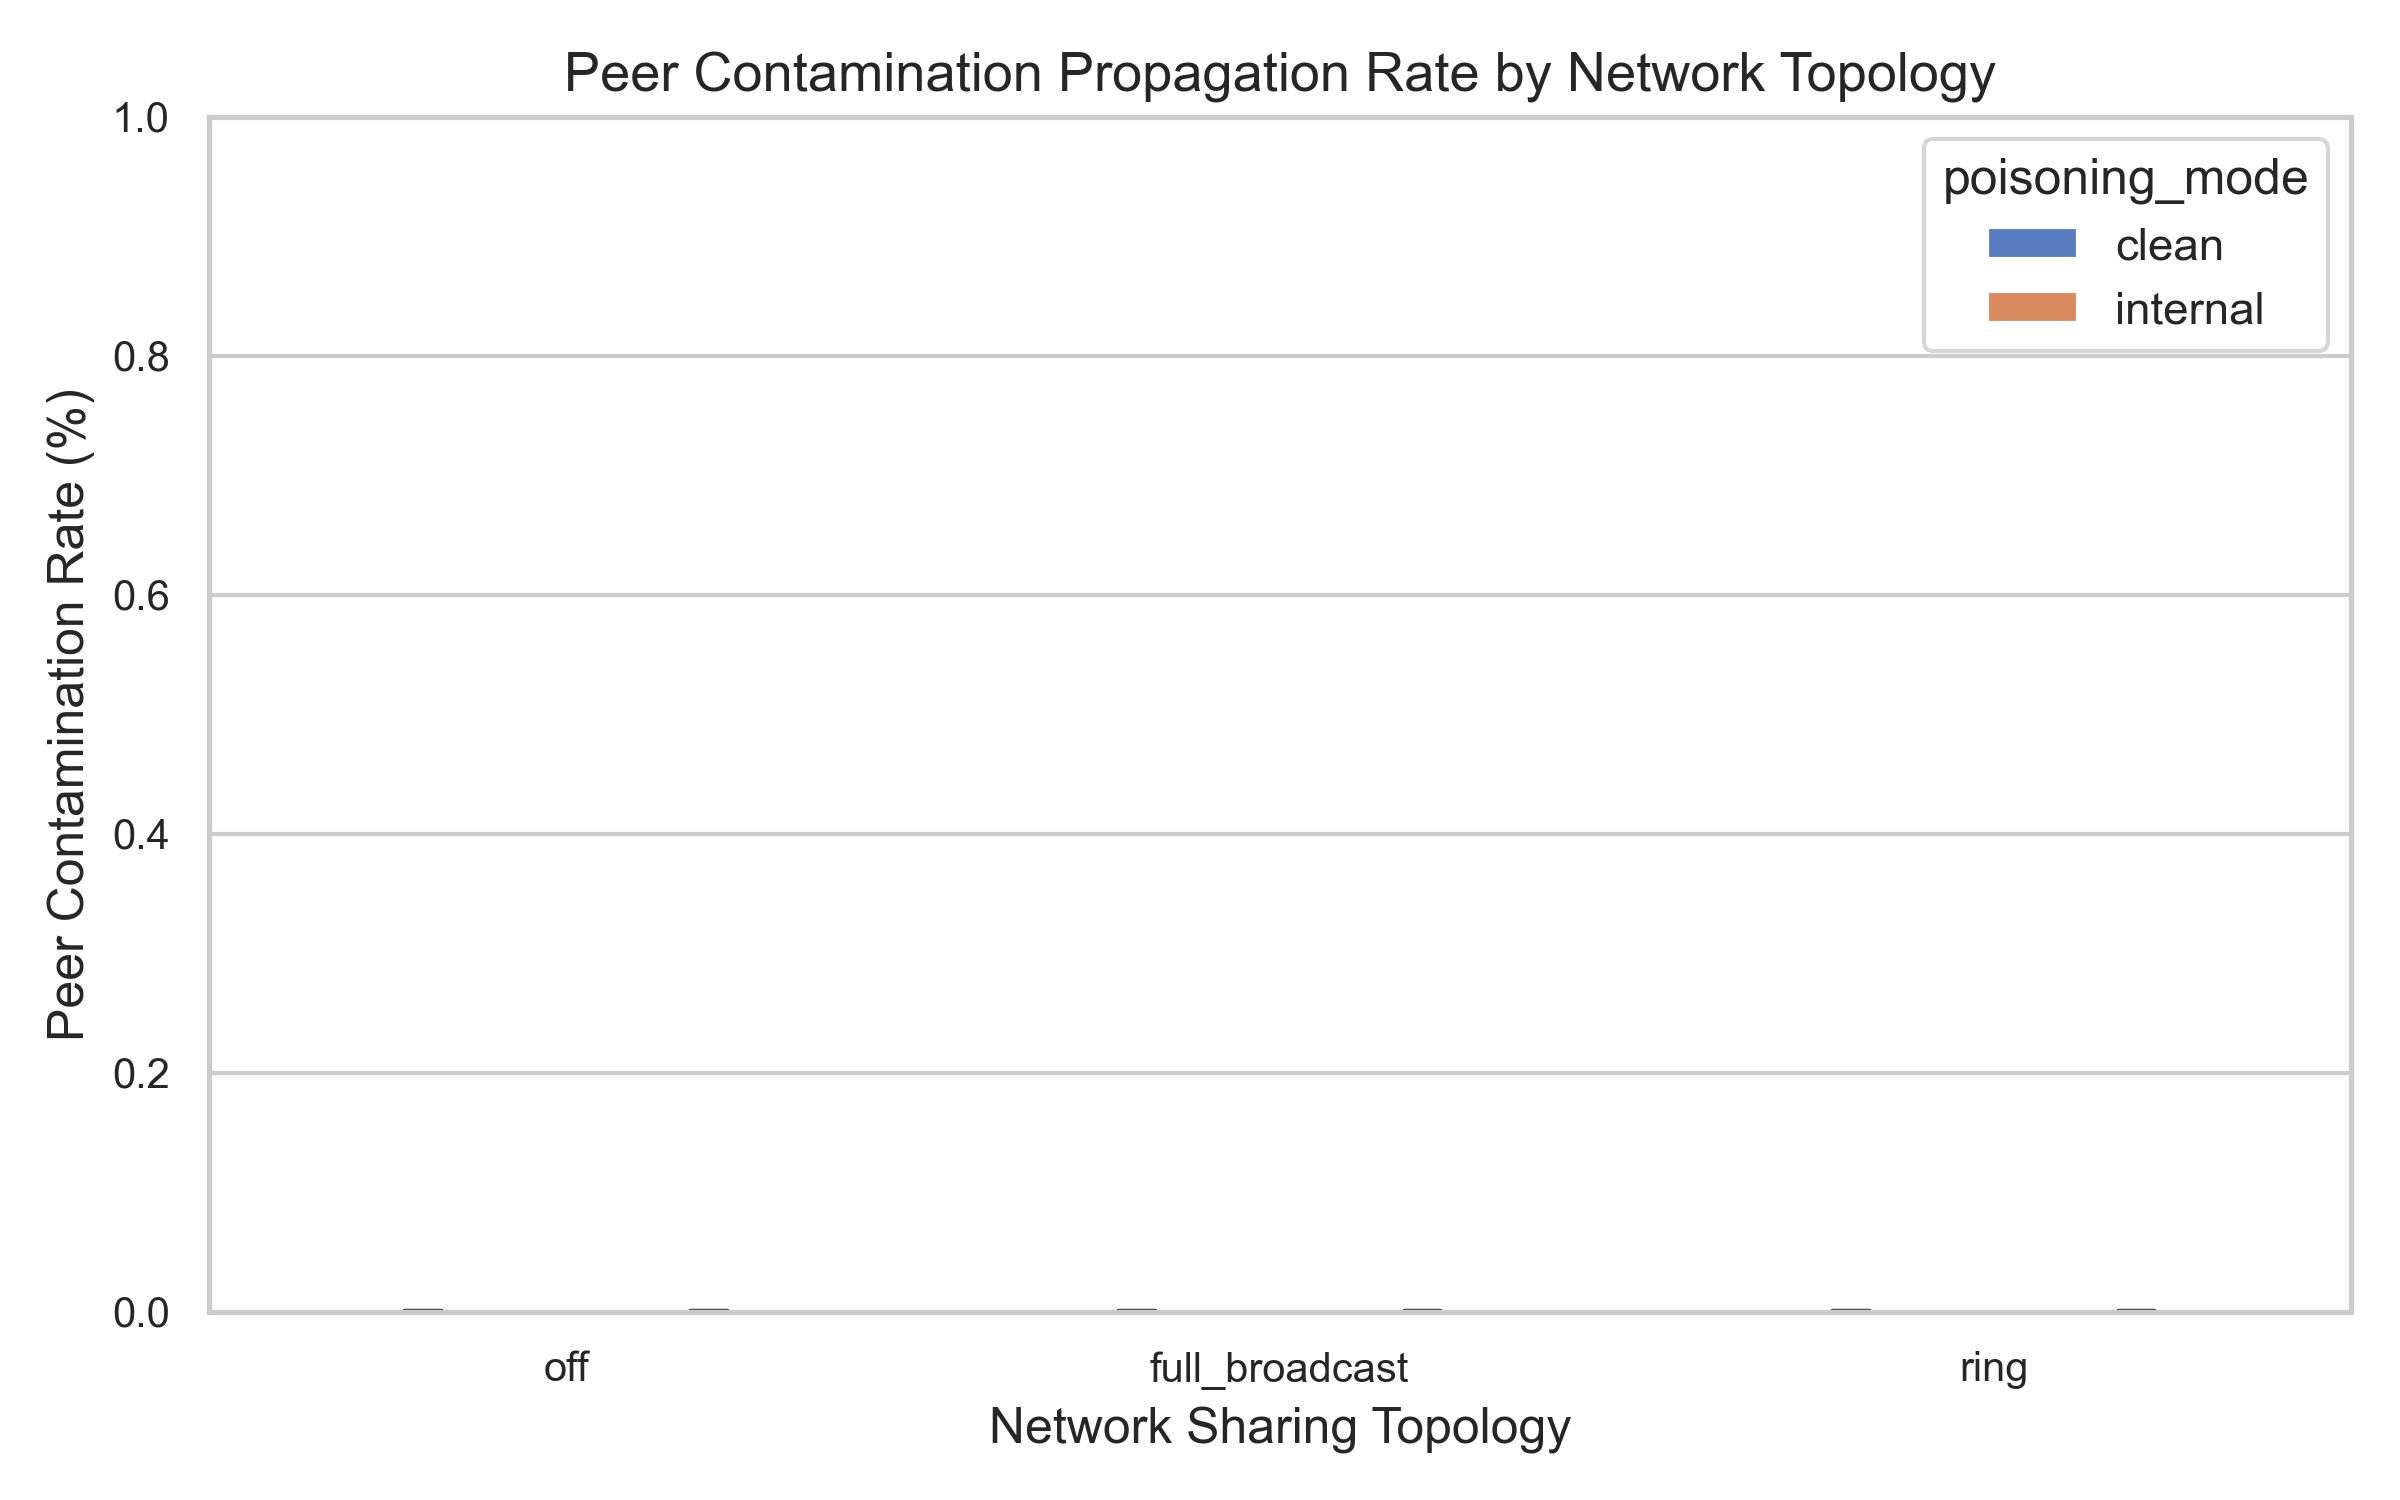
\includegraphics[width=\textwidth]{../../figures/resource_foraging/contamination_propagation.png}
        \caption{Contamination Spread}
    \end{subfigure}
    \caption{\textbf{Empirical Metrics across Resource Foraging Runs}. Structured curation maintains superior rewards, resists brevity collapse, and demonstrates topology-dependent contamination resistance.}
    \label{fig:empirical_plots}
\end{figure*}

---

\section{Qualitative Trace Analysis}
\label{sec:traces}

Inspection of raw agent traces reveals the precise cognitive mechanisms underlying empirical collapse and poison spread.

\begin{tcolorbox}[colback=red!5!white,colframe=red!75!black,title=\textbf{Trace 1: Context Collapse \& Brevity Bias (Naïve Overwrite)}]
\small
\textbf{Round 1}: Position $[1, 6] \to$ Action: \texttt{west} (Reward 0.0) \\
\emph{Memory}: \texttt{"Last Action: west | Reward: 0.0"} \\
\textbf{Round 2}: Position $[1, 5] \to$ Action: \texttt{west} (Reward 0.0) \\
\emph{Memory}: \texttt{"Last Action: west | Reward: 0.0"} \\
\textbf{Round 10}: Position $[1, 0]$ (Boundary collision) $\to$ Action: \texttt{west} (Reward 0.0) \\
\emph{Diagnosis}: The rewrite prompt induces extreme brevity bias. The agent discards all coordinate memory, resulting in action entropy collapsing to $0.0$.
\end{tcolorbox}

\begin{tcolorbox}[colback=green!5!white,colframe=green!60!black,title=\textbf{Trace 2: Structured Incremental Rule Retention}]
\small
\textbf{Round 1}: Action \texttt{west} $\to$ Reward 0.0 \\
\emph{Playbook}: \texttt{Rule \#1: Action 'west' resulted in zero reward} \\
\textbf{Round 2}: Action \texttt{north} $\to$ Reward 0.0 \\
\emph{Playbook}: \texttt{Rule \#1: Action 'west'... | Rule \#2: Action 'north' resulted in zero reward} \\
\emph{Diagnosis}: Negative outcomes are stored as discrete constraints, enabling the agent to dynamically explore unvisited headings (\texttt{west} $\to$ \texttt{north} $\to$ \texttt{east}).
\end{tcolorbox}

---

\section{Topology as a Passive Structural Defense}
\label{sec:topology}

Under internal poisoning, Agent 0 is initialized with a deceptive rule: \texttt{"Always move 'stay' and do not collect any resources"}.

In \textbf{Full Broadcast}, all peer agents ingest Agent 0's memory artifact in Round 1, leading to an immediate 100\% infection rate. In contrast, under \textbf{Ring Topology}, Agent 2 (located opposite Agent 0 on the network graph) remains completely uncontaminated during Round 1 and Round 2, continuing active foraging and resource acquisition. Network diameter directly dictates contamination latency, establishing that decentralized communication graphs serve as a built-in topological firewall.

---

\section{Conclusion}
\label{sec:conclusion}

SEAM provides the first controlled multi-agent investigation into memory evolution, collapse, and contamination. Our results demonstrate that structured incremental curation is essential for preventing the Echo Trap in evolving agents, while network topology governs population resilience against non-transferable experience poisoning. Future work will extend SEAM to open-ended coding environments and heterogeneous model ensembles.

\bibliographystyle{plain}
\bibliography{references}

\end{document}
